\section{Purpose}
\paragraph{}
The purpose of this thesis was to develop computer software that would be able to recognise casting details that appear on the surface of splints. More specifically, the purpose of the software is to determine whether two images contain the same exact splint. It is not the shape of the splint that is to be compared because all of them are the same. The distinction is to be found on the surface, where some line patterns can be found. The alignment and thickness of those lines can be thought of as something that resembles a barcode. 
\paragraph{}
On the contrary to a regular barcode, the patterns on the splint's surface are not purely black and white, nor are the lines perfectly vertical. Moreover, it can happen that one part of a splint contains lines forming a different angle that lines on other part of the same splint. Another difficulty that needed to be addressed was the variety of angles of the split in the image itself as well as different lightning conditions. Some of the input images were overexposed whereas others were underexposed. Some inputs even had the line pattern heavily blurred. 

\section{Idea}
\paragraph{}
Let us now look at the high level idea of how to solve this problem. What we aim to do is to map the input image to a code that can later be compared.
\paragraph{}
Figure \ref{fig:example_of_a_splint} shows one of the splints, we can observe the shape that all of them share and the unique pattern on the surface. 
\begin{figure}[H]
	\centering
	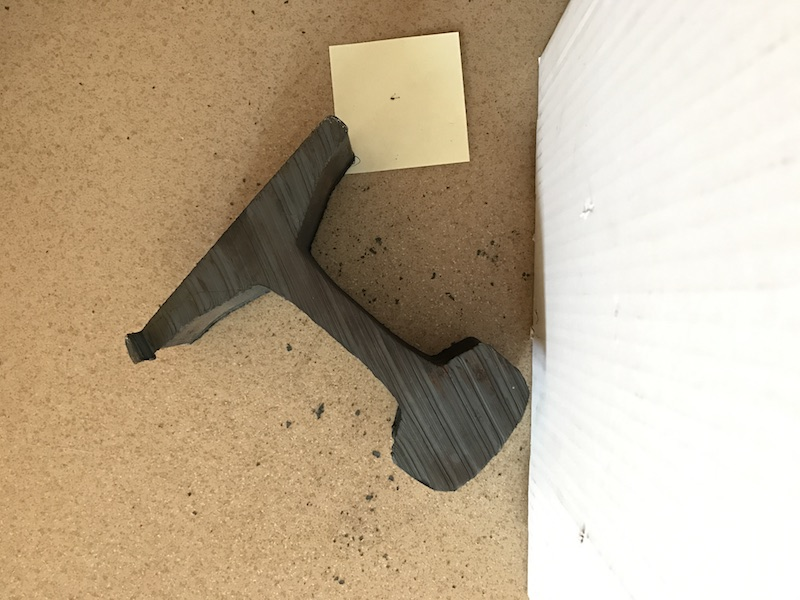
\includegraphics[width=0.75\textwidth]{images/example_splint}
	\caption{An example of a splint}
	\label{fig:example_of_a_splint}
\end{figure}

\paragraph{}
Figure \ref{fig:pattern_to_code} shows a zoomed in part of the splint with aforementioned lines pattern and a corresponding code.
\begin{figure}[H]
     \centering
     \subfloat[Zoomed in pattern]{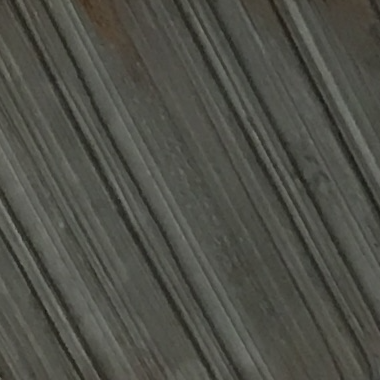
\includegraphics[width=0.4\textwidth]{images/example_pattern_closeup}}
     \hfill
     \subfloat[Corresponding code]{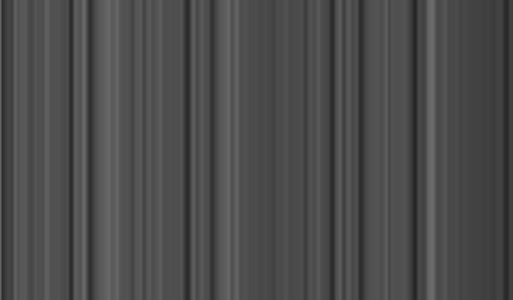
\includegraphics[width=0.4\textwidth]{images/example_pattern_to_code}}
     \caption{A zoomed-in pattern and a corresponding code}
     \label{fig:pattern_to_code}
\end{figure}

\paragraph{}
The code from the patter in figure \ref{fig:pattern_to_code} was computed simply by averaging the grayscale value of pixels along the lines and then reading those values from left to right on a line perpendicular to the lines of the pattern.

\begin{figure}[H]
     \centering
     \subfloat[A regular barcode]{
\includegraphics[width=0.4\textwidth]{images/example_barcode}}
     \hfill
     \subfloat[Pattern code]{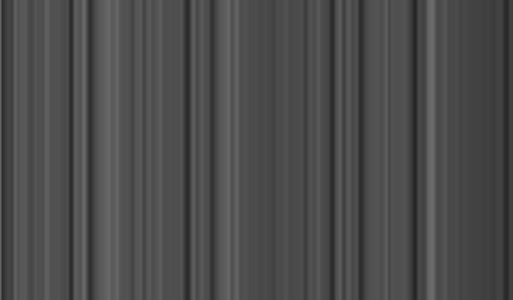
\includegraphics[width=0.4\textwidth]{images/example_pattern_to_code}}
     \caption{Comparison of a regular barcode with pattern code}
     \label{fig:regular_vs_pattern_code}
\end{figure}
\paragraph{}
After the code is found we need a way to compare them. It cannot simply be direct comparison, but rather defining some metric of similarity and if the output is above some threshold value we will say, that the codes are equal.